\documentclass[a4paper,reprint,nofootinbib,aps,pra]{revtex4-1}

\usepackage[english]{babel}
\usepackage[utf8x]{inputenc}
\usepackage[T1]{fontenc}                                               %extra characters
\usepackage{graphicx}                                                  %include graphics
\usepackage{float}                                                     %using H,h etc. to position floats
\usepackage[colorlinks = true, citecolor=blue]{hyperref}               %references are coloured and correctly sends reader to label
\usepackage{color}                                                     %coloured text width fx. {\color{red} text}
\usepackage{booktabs}                                                  %extra table tools
%\usepackage{physics}		                                       %physics package
%\usepackage{siunitx}	                                               %\SI{<tal>}{<enhed>}, \si{<enhed>}
\usepackage{amsmath}
%\numberwithin{equation}{section}                                       %equations have section number as well
\usepackage{amssymb}
\usepackage{bm}                                                        %bold font in math \bm{}
\usepackage{mathtools}                                                 %extra maths
\mathtoolsset{showonlyrefs = true}                                     %only numbers equations etc. if they are referenced to
\usepackage{cancel}                                                    %\cancel{} crosses out parts of equation
%\usepackage{tensor}                                                    %\indices{^a_b^{cd}_e} for tensor notation, * gives collapse
\usepackage{tikz}                                                      %drawing figures
\usepackage[font=small,labelfont=bf,textfont=it]{caption}              %caption formatting
\raggedbottom                                                          %helps to fix bottom (most of the time)
\setlength\parindent{0pt}                                              %Ingen indents
\usepackage{lipsum}                                                    %Import ipsum by \lipsum[1-150]

%\begin{figure}[H]
%    \centering
%    \includegraphics[width=0.5\textwidth]{picture.jpg}
%    \caption{Caption.}
%    \label{fig:label}
%\end{figure} 

%\begin{table}[]
%\begin{tabular}{|l|l|}
%\hline
%A & 25  \\ \hline
%E (MeV) & 31.28 \\ \hline
%\end{tabular}
%\caption{Caption.}
%\label{tab:my-table}
%\end{table}


\begin{document}
\title{Interpolation}
\author{Anton Rindom}


\maketitle

Here are some plots showing my implementation of a linear interpolation, and comparing it with the gsl implementation.
The function I used to generate 20 data points (from 0 to 19) was $sin(x) \cdot exp(-x / 5)$. 

% Linear interpolation plot
\begin{figure}[H]
    \centering
    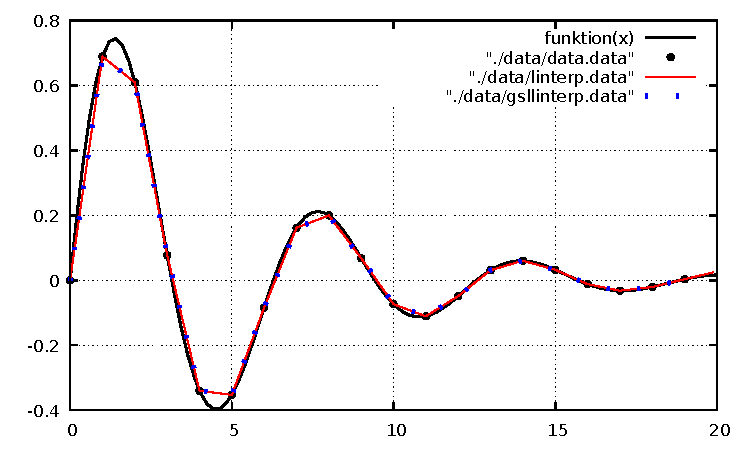
\includegraphics[width=0.5\textwidth]{./tex/linterp.pdf}
    \caption{The linear interpolation}
    \label{fig:linterp}
\end{figure} 

On figure \ref{fig:linterp} we see the linear interpolation. There's not much of interest there.
The interpolation is good on intervals where the 2nd derivative of the graph isn't too big, but fails at points, such as the first "top" where the 2nd derivative is large.
The GSL implementation is added for comparison, and as can be seen, it's right on top of my implementation.
% Integrated linear interpolation plot
\begin{figure}[H]
    \centering
    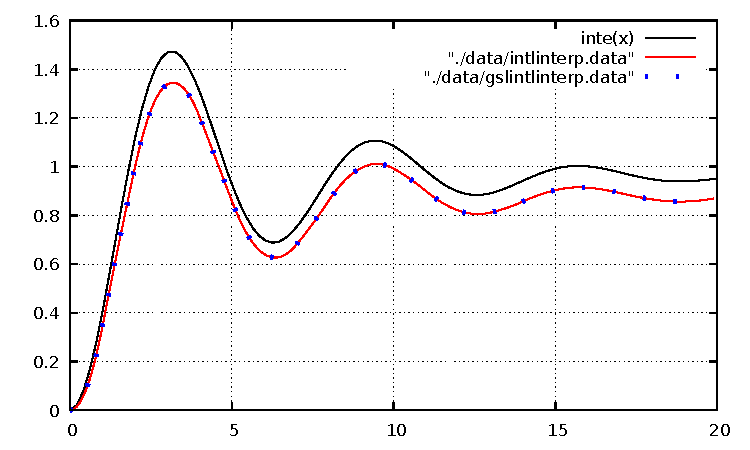
\includegraphics[width=0.5\textwidth]{./tex/intlinterp.pdf}
    \caption{The integral of the linear interpolation}
    \label{fig:intlinterp}
\end{figure} 

On figure \ref{fig:intlinterp} we see the integration (from $0$ to $x$) of the linear interpolation compared to the analytic integral.
The places on figure \ref{fig:linterp} where the interpolation doesn't match up exactly, contributes to an error in the value of the integral.

% Quadratic interpolation plot
\begin{figure}[H]
    \centering
    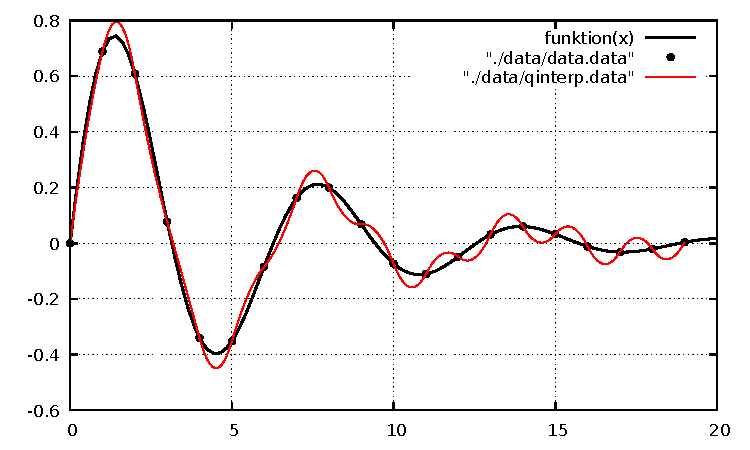
\includegraphics[width=0.5\textwidth]{./tex/qinterp.pdf}
    \caption{The quadratic interpolation}
    \label{fig:qinterp}
\end{figure} 

On figure \ref{fig:qinterp} we see the quadratic interpolation, and we can note ourselves that it oscillates quite rapidly. And so for most points it would actually be more precise to use the linear interpolation. But at certain places, where the 2nd derivative of the function is large, such as the first "top", the quadratic interpolation seems better.


\begin{figure}[H]
    \centering
    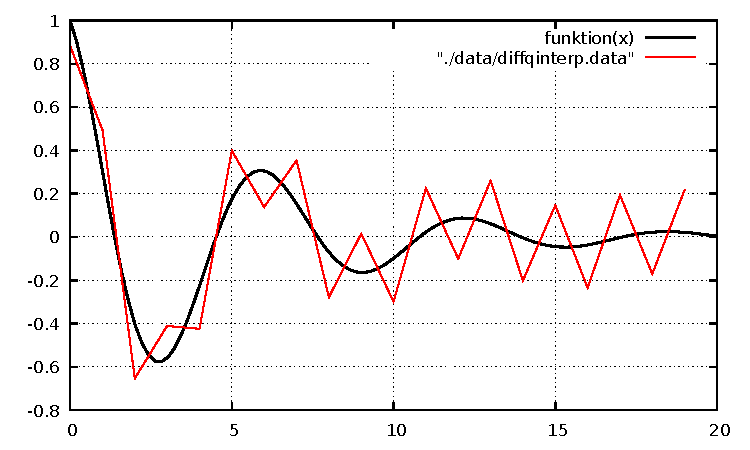
\includegraphics[width=0.5\textwidth]{./tex/diffqinterp.pdf}
    \caption{The derivative of the quadratic interpolation}
    \label{fig:diffqinterp}
\end{figure} 


On figure \ref{fig:diffqinterp} one see the derivative of the quadratic interpolation. It is continous, but not smooth, which is expected.
But it still follows the analytic derivative somewhat nicely.

\begin{figure}[H]
    \centering
    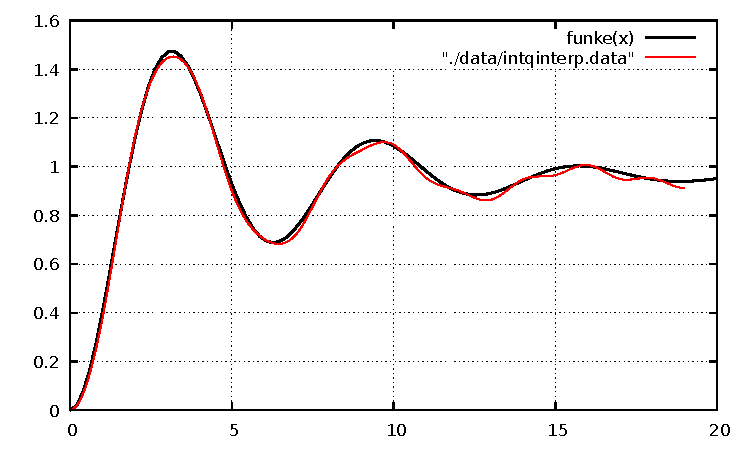
\includegraphics[width=0.5\textwidth]{./tex/intqinterp.pdf}
    \caption{The integral of the quadratic interpolation}
    \label{fig:intqinterp}
\end{figure} 

On figure \ref{fig:intqinterp} we see the integral of the quadratic interpolation, and we can especially see how the integral here is much more precise than what it was for the linear interpolation.
At the end of the graph we see, though, the small oscillations that is a symptom of the quadratic interpolation.

\begin{thebibliography}{}
\bibitem{Book} Zelevinsky \& Volya, Wiley 2017.  "Physics of Atomic Nuclei".

\end{thebibliography}

\end{document}


